\documentclass[11pt, a4paper]{book} %A4 is overruled by the geometry package later
\usepackage{geometry} \setlength{\paperwidth}{17cm}\setlength{\paperheight}{24cm} % change a4 sizes to thesis-size
% Color
\usepackage[usenames, dvipsnames]{xcolor} % color package
% Graphics
\usepackage{graphicx,amsmath,amssymb}
\usepackage{epstopdf, epsfig} % To convert eps image files to pdf
\usepackage[font=small]{caption} 
% References and links
% author-year citation
%\usepackage{natbib}
%\bibliographystyle{abbrvnat}
%\setcitestyle{authoryear,open={(},close={)}} %Citation-related commands
% natbib with compression -- does not support backref
\usepackage[square, numbers, sort&compress, comma]{natbib}
\bibliographystyle{unsrtnat}

%\usepackage[square, numbers, sort, comma]{natbib}
%\bibliographystyle{unsrtnat}


\definecolor{MyBlue}{rgb}{0,0,0.45} %color used for clickable links and so on
\definecolor{Myfig}{rgb}{0.45,0,0} %color used for clickable links and so on
\usepackage[colorlinks=true, urlcolor=MyBlue, linkcolor=MyBlue, plainpages=false, citecolor=MyBlue,bookmarks=true,bookmarksopen=true,bookmarksnumbered=true, pagebackref=true]{hyperref}
\renewcommand*{\backref}[1]{}  
    \renewcommand*{\backrefalt}[4]{
      \ifcase #1 
          {}%Cited on page #2. %No cited.
      \or
          Cited on page #2.
      \else
          Cited on pages #2.
      \fi} 
\usepackage{bookmark}    

\newcommand*\red{\textcolor{Myfig}}
%\usepackage[amssymb]{SIunits} % SI-units
\usepackage[nottoc]{tocbibind} % include or not include elements in TOC
\usepackage{lscape} % landscape page
\usepackage[figuresright]{rotating}
\usepackage{afterpage}
\usepackage[pagecolor=none]{pagecolor}
\usepackage{placeins} % floatbarrier
\usepackage{framed} %for quotes and stuff
\usepackage{siunitx}

\newcommand{\makered}[1]{\textcolor{Myfig}{#1}}  %used to insert red text

\newcommand{\publink}[1]{\href{#1}{\texttt{[Link]}}}  %used for adding links in mono-spaced font

\newcommand{\revV}[1]{\textcolor{black}{#1}}
\newcommand{\revP}[1]{\textcolor{black}{#1}}
\newcommand{\revVP}[1]{\textcolor{black}{#1}}

%\setlength{\parindent}{0mm}   %new environment that is a packed version of an itemize, useful for lists in the bio...
\newenvironment{packeditemize}{
\begin{itemize}
  \setlength{\itemsep}{1pt}
  \setlength{\parskip}{0pt}
  \setlength{\parsep}{0pt}
}{\end{itemize}}


\renewcommand{\thefootnote}{\ifcase\value{footnote}\or{$\circ$}\or{$\odot$}\or{$\circledcirc$}\or{$\circledast$}\or($\infty$)\fi} %change footnotes from daggers/stars or numbers to circular shapes

\usepackage[md]{titlesec}

\usepackage[thumblink=none,linefill=dots,height=auto,minheight={33pt},%
width={30pt},distance={10mm},topthumbmargin=auto,bottomthumbmargin=auto,%
nophantomsection=true,ignorehoffset=true,ignorevoffset=true,final=true,%
hidethumbs=false,verbose=true]{thumbs}

% Wanted appendices after every chapter
\usepackage{appendix}
\AtBeginEnvironment{subappendices}{%
	\chapter*{Appendix}
	\addcontentsline{toc}{chapter}{Appendices}
	\counterwithin{figure}{section}
	\counterwithin{table}{section}
}

%\definecolor{ColorDropImpact}{rgb}{0.99,0.88,0.57}
%\makeatletter
%\usepackage{xpatch}
%\xpatchcmd{\part}{\thispagestyle{plain}}
%{\pagecolor{ColorDropImpact}\thispagestyle{plain}}{}{}
%\xpatchcmd{\@endpart}{\vfil\newpage}{\vfil\newpage
%	\pagecolor{white}}{}{}
%\makeatother

\newcommand{\thesistitle}{Viscous Free-Surface Flows}
\newcommand{\thesistitledutch}{Viskeuze Stromingen bij Vrije-Oppervlakken}
\renewcommand{\bibname}{References}

% For 130 mm textwidth
% Whitespace on each side (non-text/non-figure) is approximately 2 cm each.
\setlength{\hoffset}{-0.55cm}  %thesis margins and offsets %don't touch these
\setlength{\textwidth}{13.0cm}
\setlength{\textheight}{18.5cm}
\setlength{\voffset}{-0.8cm}
\setlength{\headheight}{0.5cm}
\setlength{\headsep}{0.8cm}
\setlength{\footskip}{1cm}
\setlength{\oddsidemargin}{0cm}
\setlength{\evensidemargin}{0cm}

%% For 135 mm textwidth
%\setlength{\hoffset}{-0.75cm}  %thesis margins and offsets %don't touch these
%\setlength{\textwidth}{13.5cm}
%\setlength{\textheight}{18.5cm}
%\setlength{\voffset}{-0.8cm}
%\setlength{\headheight}{0.5cm}
%\setlength{\headsep}{0.8cm}
%\setlength{\footskip}{1cm}
%\setlength{\oddsidemargin}{0cm}
%\setlength{\evensidemargin}{0cm}

\setcounter{tocdepth}{1} %set depth of the table of contents


% Commands
\newcommand{\Wef}{\mathit{We}_\mathit{f}}
\newcommand{\Cas}{\mathit{Ca}_\mathit{s}}
\newcommand{\Can}{\mathit{Ca}}
%% Oh numbers
\newcommand{\Ohn}{\mathit{Oh}}
\newcommand{\Ohd}{\mathit{Oh}_\mathit{d}}
\newcommand{\Ohc}{\mathit{Oh}_\mathit{d,c}}
\newcommand{\Ohs}{\mathit{Oh}_\mathit{s}}
\newcommand{\Ohf}{\mathit{Oh}_\mathit{f}}
\newcommand{\Oha}{\mathit{Oh}_\mathit{a}}

\newcommand{\gammaaf}{\gamma_\mathit{af}}
\newcommand{\gammasf}{\gamma_\mathit{sf}}
\newcommand{\gammasa}{\gamma_\mathit{sa}}
\newcommand{\Ren}{\mathit{Re}}
\newcommand{\Wen}{\mathit{We}}
\newcommand{\Bon}{\mathit{Bo}}
\newcommand{\Boc}{\mathit{Bo}_\mathit{c}}

%% todonotes
\usepackage[obeyFinal,colorinlistoftodos]{todonotes}
\tikzset{notestyleraw/.append style={align=center}}

% todonotes specific macros begin!
\definecolor{Ch1}{HTML}{aacfed}
\newcommand{\todoChOne}[2]{\todo[color=Ch1!60, #1]{#2}}

\definecolor{Ch2}{HTML}{abceec}
\newcommand{\todoChTwo}[2]{\todo[color=Ch2, #1]{#2}}

\definecolor{Ch3}{HTML}{c9eaf6}
\newcommand{\todoChThree}[2]{\todo[color=Ch3, #1]{#2}}

\definecolor{Ch4}{HTML}{d1ecee}
\newcommand{\todoChFour}[2]{\todo[color=Ch4, #1]{#2}}

\definecolor{Ch5}{HTML}{c6e6dc}
\newcommand{\todoChFive}[2]{\todo[color=Ch5, #1]{#2}}

\definecolor{Ch6}{HTML}{e5f2e0}
\newcommand{\todoChSix}[2]{\todo[color=Ch6, #1]{#2}}

\usepackage{lipsum}

\begin{document}

\frontmatter  %start front matter

\thispagestyle{empty}
\vspace{6cm}
\begin{center}
{\huge \thesistitle}\\
\vspace{6cm}
{\large Vatsal Sanjay}  %Entire Full Name written out e.g.: Vatsal Sanjay
\end{center}


\newpage
\thispagestyle{empty}
\noindent \textbf{Graduation committee members:} \\
%Prof. Dr. Devaraj van der Meer (chairperson) \hfill University of Twente, Enschede\\
%Prof. Dr. rer. nat. Dr. h. c. Detlef Lohse (promotor) \hfill University of Twente, \\ 
%\phantom{Prof. Dr. rer. nat. Dr. h. c. Detlef Lohse (promotor)} \hfill Enschede \\
%Prof. Dr. David Qu{\'e}r{\'e} \hfill ESPCI \& Ladhyx, Paris \\
%Prof. Dr. Ir. E. Harald van Brummelen \hfill Eindhoven University of Technology, \\
%\phantom{Prof. Dr. Ir. E. Harald van Brummelen}\hfill Eindhoven\\
%Prof. Dr. Ir. Wilko Rohlfs \hfill University of Twente, Enschede \\
%Prof. Dr. Marjolein van der Linden  \hfill University of Twente, Enschede \\
%Assist. Prof. Dr. Maziyar Jalaal \hfill University of Amsterdam, Amsterdam \\
Prof. Dr. Jennifer L. Herek (chairperson) \hfill University of Twente\\
Prof. Dr. rer. nat. Dr. h. c. Detlef Lohse (promotor) \hfill University of Twente\\ 
%\phantom{Prof. Dr. rer. nat. Dr. h. c. Detlef Lohse (promotor)} \hfill Enschede \\
Prof. Dr. David Qu{\'e}r{\'e} \hfill ESPCI \& Ladhyx\\
Prof. Dr. Ir. E. Harald van Brummelen \hfill Eindhoven University of Technology\\
%\phantom{Prof. Dr. Ir. E. Harald van Brummelen}\hfill Eindhoven\\
Prof. Dr. Ir. Wilko Rohlfs \hfill University of Twente\\
Prof. Dr. Marjolein van der Linden  \hfill University of Twente\\
Assist. Prof. Dr. Maziyar Jalaal \hfill University of Amsterdam\\
\vspace{2mm}

{\centering\includegraphics[height=30mm]{fig/LogoPage_v1.eps}}

\vspace{2.5mm}

\noindent The work in this thesis was carried out at the Physics of Fluids group of the Faculty of Science and Technology of the University of Twente. This thesis was financially supported by the ERC Advanced Grant No. 740479-DDD.\\
\vspace{2mm}\\
\noindent Dutch title: \\
\noindent\emph{\thesistitledutch}\\
\vspace{2mm}\\
\noindent Publisher:\\
Vatsal Sanjay, Physics of Fluids, University of Twente,\\
P.O. Box 217, 7500 AE Enschede, The Netherlands\\
\url{https://www.vatsalsanjay.com}\\
Printed by: Gildeprint
\vspace{2mm}\\
\noindent Copyright \copyright~2022 Vatsal Sanjay. All rights reserved.\\

\noindent No part of this work may be reproduced or transmitted for commercial purposes, in any form or by any means, electronic or mechanical, including photocopying and recording, or by any information storage or retrieval system, except as expressly permitted by the author.\\

\noindent ISBN: \href{https://doi.org/10.3990/1.9789036554077}{\texttt{978-90-365-5407-7}}\\
\noindent DOI: \href{https://doi.org/10.3990/1.9789036554077}{\texttt{10.3990/1.9789036554077}}

\newpage
\thispagestyle{empty}
\vspace{1cm}
\begin{center}
{\Large \textsc{\thesistitle}}

\vspace{1cm}

DISSERTATION\\

\vspace{10mm}
to obtain\\
the degree of doctor at the Universiteit Twente,\\
on the authority of the rector magnificus,\\
prof. dr. ir. A. Veldkamp,\\
on account of the decision of the Doctorate Board,\\
to be publicly defended\\
on Friday the 15th of July 2022 at 12:45\\

\vspace{0.5cm}
by

\vspace{0.5cm}

Vatsal Sanjay\\
%\vspace{1cm}
Born on the 5th of February 1996\\
%\vspace{1cm}
in RS Tank Laheriasarai, Bihar, India\\

\newpage
\thispagestyle{empty}

This dissertation has been approved by the promotor:\\
\vspace{0.5cm}
Prof. Dr. rer. nat. Dr. h. c. Detlef Lohse

\newpage
\thispagestyle{empty}

To Anjali,\\
%\vspace{0.5cm}
the one constant of my life.
\newpage
\thispagestyle{empty}

\includegraphics{fig/My_PhD_thesis_insideBarCode.eps}
\end{center}  %include front matter file (everything before the table of contents
%
\cleardoublepage \pagenumbering{roman}  \pdfbookmark[1]{Contents}{contents}  \tableofcontents \cleardoublepage  
%start at correct side of left/right pages, change numbering to roman numerals (I II III IV), start TOC, clear double page, change page numbers to arabic numbers (1234)
\pagenumbering{arabic} \setcounter{page}{1} %set the counter to 1
%
\mainmatter

%\addthumb{Chapter  0}{\huge{\textbf{\arabic{chapter}}}}{white}{gray}
\input{0_Introduction/index}
\stopthumb
%
\part{Drop Impact}\label{PartA}
%
%%\addthumb{Chapter  1}{\huge{\textbf{\arabic{chapter}}}}{white}{gray}
%%\input{1_ChDropBetaMax/index}
%%
\addthumb{Chapter  2}{\huge{\textbf{\arabic{chapter}}}}{black}{Ch1}
\input{2_ChDropForces/index}  %Done
%
\addthumb{Chapter  3}{\huge{\textbf{\arabic{chapter}}}}{black}{Ch2}
\input{3_ChDropViscousBouncing/index}
%
\addthumb{Chapter  4}{\huge{\textbf{\arabic{chapter}}}}{black}{Ch3}
\input{4_ChDropBouncingOnFilm/index}
%
\addthumb{Chapter  5}{\huge{\textbf{\arabic{chapter}}}}{black}{Ch4}
\input{5_ChDropOnDrop/index}  %Done
%
\stopthumb
%
\part{Retraction \& Bursting}\label{PartB}
%
\addthumb{Chapter  6}{\huge{\textbf{\arabic{chapter}}}}{black}{Ch5}
\input{6_ChTaylorCulick/index} %Done
%
\addthumb{Chapter  7}{\huge{\textbf{\arabic{chapter}}}}{black}{Ch6}
\input{7_ChBurstingBubbleVP/index}
%
\stopthumb

\bookmarksetup{startatroot}% this is it
\addtocontents{toc}{\bigskip}% perhaps as well

\input{0_Conclusion/index}

%
%\nocite{*}
\bibliography{biblioClean_v12}
%

\backmatter
\chapter{Summary}

This thesis investigates several free-surface phenomena to illustrate the role of viscous stresses. In part~\ref{PartA} (chapters~\ref{chap:DropForces}--\ref{chap:DropOnDrop}), we study the impact of spherical liquid drops on non-wetting substrates, while in part~\ref{PartB} (chapters~\ref{chap:TaylorCulick}--\ref{chap:BurstingBubbleVP}), we focus on capillary-driven retraction of films and bursting of free-surface bubbles. 

In \textbf{chapter~\ref{chap:DropForces}}, we study water drops impacting non-wetting substrates and find that not only is the inertial shock at impact associated with a distinct peak in the temporal evolution of the normal force, but so is the jump-off, which was hitherto unknown. Furthermore, the inertial pressure force sets the magnitude of both these peaks in the normal reaction force. Surprisingly, some low-velocity impacts can lead to a remarkably high second peak in the normal force, which can even be three times larger than the first. This enhancement can be attributed to the collapse of an air cavity inside the liquid drop leading to singular Worthington jets. Our results thus give a fundamental understanding of the drop impact dynamics on a non-wetting surface and the forces associated with it. Such insight is crucial to developing countermeasures to the failure of superhydrophobicity in technological applications (for example, by avoiding the regime with high impact forces).

In \textbf{chapter~\ref{chap:DropViscousBouncing}}, we delineate the bouncing to the non-bouncing transition of drops falling on a non-wetting substrate. Throughout the drop impact process, viscous dissipation enervates internal momentum. A drop will cease bouncing and stay on the substrate if its upward momentum (driven by capillarity and resisted by viscous stresses) after the drop impact, spreading, and retraction process is insufficient to overcome gravity. Indeed, gravity and viscosity conspire to inhibit drop bouncing off non-wetting substrates. We further observe that close to this transition, the rebound process is independent of the impact parameters. This observation disentangles the later stages of the rebound from the initial impact dynamics. These results are helpful in applications where drop bouncing must be suppressed, for example, inkjet printing, cooling applications, pesticides application, and criminal forensics.

In \textbf{chapter~\ref{chap:DropBouncingOnFilm}}, we investigate drops bouncing off viscous liquid films that mimic atomically smooth substrates. The repellent behavior of such substrates requires the presence of an air layer trapped between the impacting drop and the liquid film. Drops impacting on viscous liquid films show two distinct bouncing regimes: (i) the substrate--independent and (ii) substrate--dependent bouncing. In the former, the impact dynamics are not affected by the presence of the viscous film owing to its high viscosity or negligible thickness. However, in the latter, both the drop and film properties influence the rebound dynamics and govern the bouncing to non-bouncing transition. On the other hand, within the substrate--independent limit, repellency is suppressed once the drop viscosity exceeds a critical value as on superamphiphobic substrates discussed in chapter~\ref{chap:DropViscousBouncing}.

In \textbf{chapter~\ref{chap:DropOnDrop}}, we find that in the presence of a non-wetting substrate, the drop-on-drop impact results in five rebound scenarios, four of which do not involve coalescence. The impacting drop lifts a lazy sessile one in two of the four rebound scenarios. If sufficient energy is transferred between the drops, both drops can take off the substrate, while in some cases, the impacting drop kicks the sessile drop off the substrate but itself cannot bounce. Furthermore, one-to-one comparisons between the experimentally and numerically determined drop boundaries and center of mass mechanical energies illustrate the power of the direct numerical simulations for quantitatively predicting the dynamics of drop-on-drop impact. Insights from chapters~\ref{chap:DropBouncingOnFilm} and~\ref{chap:DropOnDrop} are essential because, for most industrial applications, such as inkjet printing or additive manufacturing, droplets are deposited on a pre-existing layer of another drop or film. Hence, the relative precision of the drop deposition and its shape evolution may decide the success or failure of these devices. 

Note that although we do direct numerical simulations of the several drop impact scenarios in chapters~\ref{chap:DropForces}--\ref{chap:DropOnDrop}, we do so using the continuum equations. Consequently, our numerical method is inadequate to predict whether or not a drop will coalesce with another drop or the substrate. We take this information from the experiments. Indeed the coalescence or non-coalescence of interfaces depends on several multi-physics aspects, including surface asperities and van der Waals forces. Prediction of such coalescence (or rupture) behaviors is beyond the scope of the present thesis. Still, one can couple a consistent molecular dynamics technique (like gas kinetic theory) with the continuum-based volume of fluid method to bridge this lacuna in our model in the future.

In \textbf{chapter~\ref{chap:TaylorCulick}}, we show that even when the surrounding medium interacts with the Taylor-Culick retraction of a film, the film still retracts with a constant velocity, provided that it is long enough to avoid finite film size and internal viscous effects. However, both the inertia and viscosity of the surroundings influence the magnitude of this constant velocity. Even when the surroundings have negligible viscosity, they still influence the retraction process through inertial (added mass-like) effects. On the other hand, for highly viscous surroundings, viscous dissipation dictates the retraction velocity scale. The exact nature of this variation depends on the geometry of the canonical configuration in question. For example, for retracting sheets submerged in a viscous oil, the retraction velocity scales with the visco-capillary velocity (i.e., the capillary number is a constant). However, the capillary number shows a power-law behavior for sheets retracting at an oil-air interface with the dimensionless viscosity (Ohnesorge number) of the surrounding viscous medium. 

To investigate Taylor-Culick retractions at a liquid-gas free-surface in chapter~\ref{chap:TaylorCulick}, we develop a precursor film-based three-fluid volume of fluid method that captures the experimentally-observed scaling behavior very well. In a broader perspective, one can use this method to elucidate several spreading phenomena, both at small and large scales, such as, drop-film interactions in the inkjet printing process and late time spreading during oil spillage, respectively. However, this numerical assumption is applicable only when it is thermodynamically favorable for one of the fluids to spread over the other fluids it comes in contact with, i.e., it has a positive spreading coefficient. Indeed, extending this method to generalized three-phase contact line motions is expected to yield interesting results. The current three-fluid model can also handle different surface tension forces for the three interfaces and can be used as a base model to incorporate multi-physical aspects, such as Marangoni flows and multicomponent systems.

In \textbf{chapter~\ref{chap:BurstingBubbleVP}}, we reveal that the influence of viscoplasticity on the capillary-driven bursting of a bubble at a liquid-gas free-surface is twofold: (i) it manifests as an increase in effective viscosity to attenuate the capillary waves that control the bursting process, and (ii) the plasticity of the medium resists any attempts to deform its free-surface. Immediately after bursting, the large capillary stresses localized at the intersection of the bubble cavity and the free-surface result in a train of capillary waves that travel down the bubble cavity. In liquids with low yield stresses, these waves still follow the same behavior as their Newtonian counterpart. Subsequently, the cavity collapse leads to a Worthington jet that might break into droplets owing to the Rayleigh-Plateau instability. However, the capillary waves and the Worthington jet vanish for liquids with a large yield stress. Furthermore, yield-stress fluids can sustain deformations. Consequently, even after waiting a long time, the cavity never returns to its zero surface energy configuration (a flat free-surface). For high yield-stress liquids, the plasticity of the medium can even overcome the capillary waves that try to yield the free surface, thus freezing a zoo of final crater shapes. 
  %summary English (obligatory)
\chapter[Samenvatting]{Samenvatting\raisebox{.3\baselineskip}{\normalsize\footnotemark}}
\footnotetext{I would like to thank Sander Huisman, Maaike Rump, and Carola Seyfert for proofreading the Dutch summary.}

%\chapter[Samenvatting]{Samenvatting}

In dit proefschrift hebben wij verschillende verschijnselen aan het vrije oppervlak onderzocht om de rol van viskeuze spanningen te illustreren. Deel~\ref{PartA} (hoofdstukken~\ref{chap:DropForces}--\ref{chap:DropOnDrop}) bestudeerde de impact van sferische vloeistofdruppels op niet-natte substraten. Deel~\ref{PartB} (hoofdstukken~\ref{chap:TaylorCulick}--\ref{chap:BurstingBubbleVP}) concentreerde zich op capillair-gedreven terugtrekking van films en het barsten van vrije-oppervlakte bellen.

In \textbf{hoofdstuk~\ref{chap:DropForces}} bestuderen we waterdruppels die inslaan op niet-natte substraten. We vinden dat zowel de impact als de take-off gepaard gaan met een toename van de impactkracht op het substraat. De traagheidsdrukkracht bepaalt de grootte van deze beide pieken in de normale reactiekracht. Maar verrassend genoeg kunnen zelfs botsingen bij lage snelheid leiden tot een opmerkelijk hoge tweede piek in de normaalkracht, die zelfs groter kan zijn (bijna driemaal) dan de eerste. Deze verbetering kan worden toegeschreven aan de ineenstorting van een luchtholte binnenin de vloeistofdruppel, wat leidt tot enkelvoudige Worthington-stralen.Onze resultaten geven dus een fundamenteel inzicht in de dynamica van de druppelinslag op een niet-bevochtigd oppervlak en de krachten die ermee gepaard gaan. Zulk inzicht is van cruciaal belang om tegenmaatregelen te ontwikkelen tegen het falen van superhydrofobiciteit in technologische toepassingen (bijvoorbeeld door het vermijden van het regime met hoge impactkrachten).

In \textbf{hoofdstuk~\ref{chap:DropViscousBouncing}} we bepalen de overgang van stuiterende naar niet-stuite\-ren\-de druppels die op een niet-nat substraat vallen. Tijdens het druppel impact proces verstoort de viskeuze dissipatie het interne momentum. Een druppel zal ophouden met stuiteren en op het substraat blijven liggen als zijn opwaartse momentum (aangedreven door capillariteit en tegengewerkt door viskeuze spanningen)  na het proces van druppelinslag, verspreiding en terugtrekking onvoldoende is om de zwaartekracht te overwinnen. Zwaar\-tek\-racht en viscositeit werken dus samen om te voorkomen dat druppels van een niet-nat substraat stuiteren. Wij stellen verder vast dat dicht bij deze overgang het terugslagproces onafhankelijk is van de inslagparameters. Deze waarneming ontkoppelt de latere fasen van de terugslag van de initi{\"e}le dynamica van de inslag. Deze resultaten zijn nuttig in toepassingen waar het terugkaatsen van een druppel moet worden onderdrukt, bijvoorbeeld bij inkjetdruk, koeltoepassingen, de toepassing van pesticiden en criminele forensische wetenschap.

In \textbf{hoofdstuk~\ref{chap:DropBouncingOnFilm}} onderzoeken we druppels die weerkaatsen op viskeuze vloeistoffilms die atomair gladde substraten nabootsen. Het afstotend gedrag van dergelijke substraten vereist de aanwezigheid van een luchtlaag opgesloten tussen de stotende druppel en de vloeibare film. Druppels die inslaan op viskeuze vloeistof films vertonen twee verschillende stuiteren regimes, namelijk het substraat-onafhankelijke en het substraat-afhankelijke stuiteren. In het eerste regime wordt de botsingsdynamiek niet be{\"i}nvloed door de aanwezigheid van de viskeuze film, als gevolg van zijn hoge viscositeit of verwaarloosbare dikheid. In het laatste echter beïnvloeden zowel de eigenschappen van de druppel als die van de film de terugstuitdynamiek. Binnen de substraatonafhankelijke grens wordt de afstoting onderdrukt zodra de druppelviscositeit een kritische waarde overschrijdt, zoals bij superamphiphobische substraten die in hoofdstuk~\ref{chap:DropViscousBouncing}. Het substraat-afhankelijke regime laat ook een grens toe voor druppels met lage viscositeit, waarin alleen de eigenschappen van de film de remming van afstoting bepalen.

In \textbf{hoofdstuk~\ref{chap:DropOnDrop}} hebben wij ontdekt dat in aanwezigheid van een niet-bevochtigend substraat, de druppel-op-druppel botsing vijf terugslagscenario's oplevert, waarvan er vier geen coalescentie inhouden. De botsende druppel tilt in twee van de vier terugspringscenario's een luie sessiele op. Als er voldoende energie tussen de druppels wordt overgedragen, kunnen beide druppels van het substraat kunnen nemen, terwijl in sommige gevallen de botsende druppel de sessiele druppel van het substraat schopt, maar zelf niet kan stuiteren. Bovendien illustreert een {\'e}{\'e}n-op-{\'e}{\'e}n vergelijking tussen de experimenteel en numeriek bepaalde druppelgrenzen en de mechanische energieën van het massamiddelpunt de kracht van de directe numerieke simulaties voor het kwantitatief voorspellen van de dynamica van druppel-op-druppel inslag. Inzichten uit de hoofdstukken~\ref{chap:DropBouncingOnFilm}  en~\ref{chap:DropOnDrop}  zijn belangrijk omdat voor de meeste industriële toepassingen, zoals inkjet printing of additive manufacturing, druppels worden afgezet op een reeds bestaande laag van een andere druppel of film. Vandaar dat de relatieve precisie van de druppelafzetting en zijn vormevolutie het succes of het falen van deze toestellen kunnen bepalen. 

Merk op dat, hoewel wij directe numerieke simulaties doen van de verschil- lende scenario’s van druppelinslagen in de hoofdstukken~\ref{chap:DropForces}--\ref{chap:DropOnDrop}, wij dat doen met behulp van de continu{\"u}mvergelijkingen. Bijgevolg is onze numerieke methode ontoereikend om te voorspellen of een druppel al dan niet met een andere druppel of met het substraat zal samensmelten. Wij halen deze informatie uit de experimenten. Het al of niet samensmelten van grensvlakken hangt namelijk af van verschillende multifysische aspecten, waaronder oppervlakte- asperiteiten en vanderwaalskrachten. Voorspelling van zulke coalescentie (of breuk) gedragingen valt buiten het bereik van dit schrift, maar men kan een consistente moleculaire dynamica techniek (zoals de gaskinetische theorie) koppelen aan de continu{\"u}m-gebaseerde vloeistofvolume methode om deze lacune in ons model in de toekomst te overbruggen.

In \textbf{hoofdstuk~\ref{chap:TaylorCulick}} vinden wij dat zelfs wanneer het omringende medium interageert met de Taylor-Culick terugtrekking van een film, de film nog steeds met een constante snelheid terugtrekt, op voorwaarde dat de film lang genoeg is om eindige filmgrootte en inwendige viskeuze effecten te vermijden.  Zowel de traagheid als de viscositeit van de omgeving beïnvloeden echter de grootte van deze constante snelheid. Voor de veralgemeende Taylor-Culick terugtrekkingen geldt dat zelfs wanneer de omringende delen een verwaarloosbare viscositeit hebben, zij toch het terugtrekproces beïnvloeden door inerti{\"e}le (toegevoegde massa achtige) effecten. Voor een zeer viskeuze omgeving daarentegen dicteert de viskeuze dissipatie de schaal van de terugtreksnelheid. De precieze aard van deze variatie hangt af van de geometrie van de canonische configuratie in kwestie. Bijvoorbeeld, voor terugtrekkende vellen ondergedompeld in een viskeuze olie, schaalt de terugtreksnelheid met de visco-capillaire snelheid (d.w.z., het capillair getal is een constante). Voor vellen die zich terugtrekken aan een olie-lucht grensvlak vertoont het capillair getal echter een power-law gedrag met de dimensieloze viscositeit (Ohnesorge getal) van het omringende viskeuze medium.

Om de Taylor-Culick terugtrekkingen aan een vloeistof-gas vrij-oppervlak te onderzoeken in hoofdstuk~\ref{chap:TaylorCulick}, ontwikkelen we een precursor film-gebaseerde drie-vloeistof vloeistofvolume methode die het experimenteel waargenomen schalingsgedrag zeer goed weergeeft. In een breder perspectief kan men deze methode gebruiken om verschillende verspreidingsfenomenen op te helderen, zowel op kleine als op grote schaal, zoals respectievelijk druppel-film interacties in het inkjet drukproces en laattijdige verspreiding tijdens olielekkage. Deze numerieke aanname is echter alleen van toepassing wanneer het thermodynamisch gunstig is voor een van de vloeistoffen om zich te verspreiden over de andere vloeistoffen waarmee het in contact komt, d.w.z. dat het een positieve verspreidingscoëfficiënt heeft. Uitbreiding van deze methode tot veralgemeende driefasige contactlijnbewegingen zal naar verwachting interessante resultaten opleveren. Het huidige drie-fasen model kan ook omgaan met verschillende oppervlaktespanningskrachten voor de drie grensvlakken en kan worden gebruikt als basismodel om multi-fysische aspecten te incorporeren, zoals Marangoni stromingen en multicomponent systemen.

In \textbf{hoofdstuk~\ref{chap:BurstingBubbleVP}}, hebben wij aangetoond dat de invloed van viscoplasticiteit op het capillair-gedreven barsten van een luchtbel aan een vloeistof-gas vrije-oppervlak tweevoudig is: (i) het manifesteert zich als een verhoging van de effectieve viscositeit om de capillaire golven te dempen die het barstproces regelen, en (ii) de plasticiteit van het medium verzet zich tegen alle pogingen om het vrije-oppervlak te vervormen. Onmiddellijk na het barsten leiden de grote capillaire spanningen, geloka- liseerd op het snijpunt van de belholte en het vrije-oppervlak, tot een trein van capillaire golven die langs de belholte naar beneden beweegt. In vloeistoffen met lage vloeispanningen volgen deze golven nog steeds hetzelfde gedrag als hun Newtoniaanse tegenhanger. Vervolgens leidt het instorten van de holte tot een Worthington straal die in druppels kan breken ten gevolge van de Rayleigh-Plateau instabiliteit. Voor vloeistoffen met een grote vloeispanning echter verdwijnen de capillaire golven en de Worthington jet. Opbrengst-druk vloeistoffen kunnen vervormingen volhouden. Bijgevolg keert de holte, zelfs na lang wachten, nooit terug naar de nulconfiguratie van de oppervlakte-energie (een vlak vrij-oppervlak). Voor vloeistoffen met hoge vloeispanning kan de plasticiteit van het medium zelfs de capillaire golven overwinnen die het vrije-oppervlak trachten op te leveren, en zo een zoo van uiteindelijke kratervormen bevriezen.
 %summary Dutch (obligatory)
\chapter{Acknowledgments}

First of all, I want to thank {\bf you}, the reader, for picking up this thesis. Thank you for reading through all the chapters, or if you are anything like me, thank you for coming straight to the acknowledgment section. Whenever I find a Ph.D. thesis, this section is my first stop. The journey of any doctoral candidate is long with all its ups and downs, which often (hopefully) culminates in a collection of chapters. Every journey is unique, and one can understand the person on this journey by knowing who they acknowledge after completing such a taxing yet inciting endeavor. My Ph.D. journey at the Physics of Fluids (PoF) group, like all others, has been made possible by the support of many people. I want to spend the next few pages sharing my gratitude towards them. 

{\bf Detlef}, thank you so much for giving me this opportunity to work with you and all the independence to pursue the wide variety of intellectually stimulating problems in this thesis. We first got in touch via email and Skype (in the old pre-pandemic, non-zoom days). I received a one-line reply to my long request seeking a research position at PoF, which I now know to be your efficient style, as these one-line emails have become a part of my daily life. I cannot express in words how much I have enjoyed working with you over the past four years. Someone once told me that working with you is like working with Albert Einstein but in fluid dynamics. After four incredible years, I can attest to this fact. I particularly enjoy our meetings when they do not have an end time. I get to hear your thoughts and learn about the rich history of fluid dynamics, which are equally inspiring. I am often amazed by your energy. For example, I remember once, while we recorded lectures for the Advanced Fluid Dynamics course, we spent almost eight hours in your office. My job was simply to hit record and listen in as you taught the modules on turbulence, boundary layers, and instabilities. It was incredibly one of the most informative sessions of my life. Even after eight hours, you were still as energetic as when we started. Indeed, that day I witnessed the perfect example of what happens when one does what they love. In your words, the only essential thing in one's life is the brain and the passion for science; everything else is just background noise. {\bf Detlef}, for all the hours that you spent with me working out the Physics, thanks a lot. I want to continue this quest in the world of fluid dynamics by asking relevant questions, as you so often told me, and answer them to the best of my abilities. I am looking forward to working ever so closely with you in the future. I have a lot yet to learn from you, and I am sure we will have many long sessions filled with intellectually stimulating discussions in the future. 

{\bf Mazi}, the transition at the beginning of anyone's Ph.D. journey is often overwhelming and confusing. Thank you for helping me through this phase. Working on chapter six of this thesis, I learned a lot about fluid dynamics and non-Newtonian flows. Furthermore, you have always lent an ear whenever I felt stuck in the past four years. The long scientific discussions and the ideas you passed on have been invaluable to me. But, of course, your influence on this thesis is not restricted to just being the go-to person for quenching Scientific curiosity. You have also acted as the perfect Yoda on this Ph.D. journey, both academically and otherwise. Thank you so much for inspiring me all through the process. I look forward to working together on many ideas and projects. 

I have been fortunate to be always surrounded by some of the most incredible mentors, {\bf Detlef}, {\bf Mazi}, {\bf St{\'e}phane Z.}, {\bf Andrea}, {\bf John S.}, {\bf Jean-Philippe}, {\bf Micka{\"e}l}, and {\bf Arup}. The privilege often reminds me of these words taken from a letter Newton wrote to Robert Hooke, \lq\lq If I have seen further, it is by standing on the shoulders of giants.\rq\rq\, I am indebted to all of you for encouraging and showing me the way. {\bf St{\'e}phane Z.}, thank you for teaching me all I know about the volume of fluid method. Given that this method forms the backbone of my entire Ph.D. thesis, it is safe to say that this thesis would not exist without the GIAN course on two-phase flow at the Indian Institute of Technology Roorkee. You are always eager to discuss science whenever we meet during conferences or during your visits to PoF. These discussions have benefited me tremendously throughout my career. {\bf Andrea}, your enthusiasm, passion, and search for new fluid dynamics problems have motivated me. The long sessions with you always leave me full of thoughts and ideas. {\bf Arup}, I would also like to thank you for introducing me to the fascinating world of fluid dynamics. The journey that started in your office about eight years ago has now reached this stage, with hopefully more to come. 

Here, I would like to take the opportunity to thank my {\bf committee members}. Thanks a lot for agreeing to be a part of my graduation committee and for spending so much of your precious time reading this thesis. I look forward to interacting with you all on the day of the defense and in the future. 

Next, I want to thank my paranymphs, {\bf UJ} and {\bf Udo}. First of all, thanks for agreeing to accompany me on the stage as I defend this Ph.D. thesis and for dressing up formally for the occasion. I know how much both of you share my discomfort in adhering to formal attire. {\bf Udo}, your passion for perfection is a force to reckon with. Thanks for always being critical of my work and providing honest feedback. We had a great time working on the Taylor-Culick retractions, which formed the largest chapter of this thesis. I hope we will continue our collaboration and the long walks that consistently contributed to pushing these collaborations. I hope we will tackle many more interesting fluid dynamics problems in the future. {\bf UJ}, I have found a great friend in you. We have spent many weekends in our offices discussing all things related to fluid dynamics and life. {\bf Yanshen}, {\bf Peter}, you, and I made the weekend warriors at PoF. We also had a wonderful and insightful time in Copenhagen. I have also always enjoyed our long walks. By the way, {\bf UJ}, we have known each other since my first visit to PoF when we went out for dinner following my interview with {\bf Detlef} where he offered me this doctoral position. Little did I know that we share a common friend, who, as it turns out, is one of my closest allies in life. Thank you, {\bf Sonali} for always being available at a phone call's notice and for all the help you have provided throughout these years.

{\bf Pierre}, we have shared an office for almost three years. We have interacted on several open projects and ideas throughout this time and often had heated but spirited discussions about our works. Collaborating with you on chapters 2 and 3 of this thesis has been excellent. I have thoroughly enjoyed our brainstorming sessions. In one of them, we also came up with the title of this thesis. In fact, the first part of this work on drop impact processes draws motivation from these discussions and your thesis. The latter has also contributed to improving my understanding of the French language. I also want to thank you for always lending an ear to my, at times, crazy ideas. 

Next, I would like to thank all my collaborators and coauthors, {\bf Claas-Willem}, {\bf Olinka}, {\bf Doris}, {\bf Jon}, {\bf Bin}, {\bf Cunjing}, {\bf Srinath}, and {\bf Pallav}. I have learned a lot from all of you and am looking forward to several stimulating collaborations in the future. 

Next, I want to thank the entire group at PoF, my professional family. The Wednesday seminars are a tour de force. We get to share ideas, listen to fluid dynamics leaders from across the globe, and most importantly, enjoy stimulating discussions. Being a part of this group is a privilege I have enjoyed as a young researcher. I want to thank {\bf Joanita} for her superhuman organizational skills. You show an ideal combination of speed and precision. Thank you for always having a solution to any and all of my problems. 

Of course, the group is only as good as the people in it. At PoF, I interacted with amazing fluid dynamicists. Where else would one find a fluid dynamics rock star like {\bf Leen} whose contributions to fluid dynamics research and several lives are both incredible and humbling. 

{\bf Devaraj}, thank you for agreeing to be the chairperson of my committee and for all the positiveness during our interactions. Your knowledge of all matters, Physics or otherwise, is terrific. I got a first-hand experience during the pop quiz at Landal Village. It was a pleasure to be a part of the team centurions and compete alongside {\bf Javier} and {\bf Lor{\'e}ne}. Indeed, it was a lovely group outing. I really enjoyed the place, the science, and most of all, the company in the bungalow \#100. Thanks a lot. 

{\bf Jacco}, thank you for the insightful conversations regarding free-surface flows. We have run into each other several times at Starbucks, and I am often intrigued by how easy it is to talk to you about everything, irrespective of the complexity. I remember the one conversation we had regarding the origin of viscosity and the no-slip boundary condition in continuum mechanics. It was, in a word, inspiring. I would also like to thank {\bf Alvaro}, {\bf Richard}, {\bf Corinna}, {\bf Dominik}, {\bf Tim}, {\bf Michel}, {\bf Marjolein}, and {\bf Christian} for always asking just the right questions during group meetings, seminars, or even at dinner tables. 

{\bf Sander}, thank you for all the chocolates that helped maintain my blood sugar level over the years. I could always rely on your (not-so) secret stash whenever I needed something. Also, thank you for giving me a chance to teach some of the Advanced Fluid Mechanics modules. The best way to learn something is to teach it, and I thank you for allowing me to gauge and sharpen my knowledge through these lectures. Lastly, thank you for proofreading the Dutch summary despite your busy schedule and for your help with making the PoF-Basilisk logo, along with all the illustrator tricks you have shown me over the years. I look forward to spending more time with you and, finally, learning Mathematica. 

{\bf Diana}, we went on several long walks together through the woods, despite being scared of the caterpillars. We also had so much fun in the pre-pandemic (almost prophetic) Pandemic games. Thank you for all the fun we had together. Also, thank you for all the relatable stories from Columbia; oops, I meant Colombia, captain correct America. 

{\bf Youssef}, we share several commonalities. We started our respective doctoral works at a gap of a few months, share the same office, and perhaps most importantly, specialize in Basilisk. Thank you for always providing a bouncing board for new and old Basilisk ideas and tricks. Now, coincidentally, we are also getting married within a few months of each other. I wish you an amazing married life. 

{\bf Maaike}, thank you for all the fun and scientific discussions we have had over the years. Thank you for always listening in with so much attention and being ever so polite. I wish you the best for your bike trip across a few continents.

{\bf Carola}, I always look forward to our coffee breaks. Thank you for all the discussions and advice you have given me throughout the years. And also, thanks a lot for allowing me to \lq steal\rq\, some of your thesis template ideas. 

{\bf Jessica}, I have always enjoyed your company. Thank you so much for all the fun and, at times, serious conversations we have had over the years.

{\bf Varghese}, {\bf Shantanu}, and {\bf Vamsi}: you formed the previous generation of doctoral candidates who graduated immediately before I joined PoF. You all were also deeply involved in my hiring interviews. Thank you for sharing your experiences and showing me what a wonderful place PoF is. There are still many PoF colleagues and friends who I would like to thank for making the last four years a delight and a blast, {\bf CS}, {\bf Yibo}, {\bf Timothy}, {\bf Robert}, {\bf Anupam}, {\bf Youan}, {\bf Morgan}, {\bf Chris}, {\bf Farzan}, {\bf Ambre}, {\bf Alex}, {\bf Martin E.}, {\bf Vanshu}, and {\bf Anja}. Thank you, {\bf Minkush} for being so kind and caring for everyone. {\bf Lijun} and {\bf Yogesh}, thank you for the several dinners we have had together and never kicking {\bf Udo} or me out even if we self-invited ourselves. I also enjoyed our cricket games together with {\bf Srinidhi}. 

My old and current office-mates: {\bf Rodrigo}, {\bf Dennis B.}, {\bf Mazi}, {\bf Martin}, {\bf Marvin}, {\bf Pierre}, and {\bf Youssef}. Thanks for always maintaining such a great environment at {\bf ME 246B}. {\bf Dennis B.}, your passion for open-source programming is unparalleled. I have always enjoyed out long discussions on this topic. 

My office neighbors, the gang in {\bf ME 24/7}: {\bf Jelle}, {\bf Pieter}, {\bf Srinidhi}, and {\bf UJ}, thank you for always providing a place to cool off and swap stories. 

Next, I would like to thank the fantastic technicians and the support team at PoF. {\bf Dennis vG.}, thank you for maintaining order at PoF. {\bf Bas} and {\bf Thomas} for helping me with all the tech support and acquiring gadgets. {\bf Gert-Wim} and {\bf Martin B.}, even though I did not participate in any experimental work during my Ph.D., it was always a delight to talk to both of you whenever we met. 

During my Ph.D., I had the privilege to engage with several motivated students, {\bf Laurence},  {\bf Coen}, {\bf Mihir}, {\bf Pim}, {\bf Steven}, {\bf Thijmen}, {\bf Tom}, {\bf Toon}, and {\bf Twan}, just to name a few. I thank you all for working with me and wish you all the best for your subsequent undertakings.

{\bf St{\'e}phane P.}, you have developed and maintained one of the largest free-software programs in our community. I started my research career with Gerris and then moved to Basilisk C. I want to thank you and the entire Basilisk community for providing a well-documented partial differential equation solver. Learning the code and implementing new modules are both very easy, thanks to your efforts.

I would be amiss if I did not mention all the love and support I have received from {\bf my family members}, including my parents, sister, and in-laws. Your willingness to support me through higher studies is commendable. In a society where graduating from college and seeking a job represent the norm, I am lucky to be associated with a family encouraging higher education. Words cannot acknowledge the support I have received from all of you. Of course, my extended family includes my fantastic close friends, {\bf Akash} and {\bf Akanksha}; thank you for always being there whenever I needed you. 

{\bf Vatsalya}, thank you for providing a sanctuary whenever I needed one and for proofreading parts of this thesis despite all the technical jargon. We have been friends since high school, and we (almost) share our first names but have pursued very different and arguably complementary career paths. My love for Physics and yours for music benefited us during high-school exams. But, I have only you to thank for introducing me to my favorite human being and now, my wife. 

{\bf Anjali}, there is nothing I can say that you do not know already. We have known each other since high school. A Physics question on Kirchhoff's circuit laws brought us together, and you have been with me ever since. You have seen me both at my best and worst. Thank you for always believing in me, even when I did not. You bring a smile to my face, irrespective of the situation. This journey would have been difficult without your constant presence in my life. My warm hugs and a big thank you to you. Thank you so much for always being there. I dedicate this thesis to you, my lovely wife and the one constant in my life. 


\chapter{About the author}
\phantom{me}\hfill 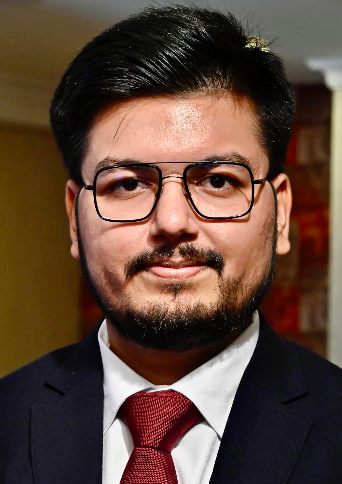
\includegraphics[height=25mm]{fig/Vatsal.pdf}\\ %latex does not supprot jpg, insert a pdf version of your profile photo if you like...
\vspace{5mm}

These are the last two pages of my Ph.D. thesis where I am supposed to write about myself. Before doing so, I must admit that it is a herculean task, but I will try my best to share my story with you.

I was born on February 5th, 1996, in Laheriasarai, a small town in Bihar, India. As a kid, my first love was reading stories, which soon became a love for history. If I were not a fluid dynamicist today, I would probably have been a historian. The only problem was that I could only read stories about others and not write one of my own, which is another of my passions. Apart from reading, I also love collecting books. Ever since childhood, I have maintained a healthy collection of books, both antique and modern. 

Thanks to one of these books, I stumbled into the fascinating world of Physics. I remember getting puzzled by a question that seemed like a paradox at the time. I still remember the question. {\it To pull a cart, a horse applies a force on it. However, Newton's third law dictates that the cart applies an equal and opposite force on the horse. If we take the horse and the cart as a system, the net force on this system is zero. Then, how does a horse pull a cart?} It took me an entire sleepless night to come up with an answer, ending in a midnight call to my secondary school Physics teacher. 

The satisfaction of coming up with the correct answer set me up on this journey which led me to do a bachelors in Mechanical Engineering from the Indian Institute of Technology Roorkee, during which I worked as an undergraduate researcher with Prof. A. K. Das in the two-phase flow lab. I also did an internship with Prof. M. Bourgoin, Prof. J-P. Matas, and Prof. J. J. Jerome. This internship introduced me to the rich European research culture and the fluid dynamics community. The style of asking questions and exploring the fundamental fluid dynamics of everyday flows appealed to me. Subsequently, I decided to switch my bachelor's program to an integrated dual degree. I finished my master's thesis with Prof. Das. These works led me to pursue a doctoral work with Prof. D. Lohse in the Physics of Fluids group, where I have spent the last four years working on this Ph.D. thesis. 

But the story is not over yet. In the future, I want to continue this quest in the world of fluid dynamics by asking relevant questions and answering them to the best of my abilities. I also want to read more books and contribute to spreading the beautiful world of fluid dynamics to everyone. One day, I would also like to run a marathon, thanks to my recently acquired love for running. 




%\include{backmatter/scientificoutput}

\cleardoublepage 

\end{document}